%%%%%%%%%%%%%%%%%%%%%%%%%%%%%%%%%%%%%%%%%%%%%%%%%%%%%%%%
%%%%%%                                            %%%%%%
%%%                                                  %%%
%      Modèle de Rapport.                              %
%               Par Matthieu Maury                     %
%                                                      %
%%%                                                  %%%
%%%%%%                                            %%%%%%
%%%%%%%%%%%%%%%%%%%%%%%%%%%%%%%%%%%%%%%%%%%%%%%%%%%%%%%%

\documentclass[10pt, a4paper]{report}

%%%%%%%%%%%%%%%%%%%%%%%%%%%%%%%%%%%%%%%%%%%%%%%%%%%%%%%%
%% Package essentiel
\usepackage[greek,english]{babel}
\usepackage[T1]{fontenc}
\usepackage{ucs}
\usepackage[utf8x]{inputenc}
\usepackage[top=2.6cm,bottom=2.6cm,right=2.1cm,left=2.1cm]{geometry}
\usepackage{float}

%%%%%%%%%%%%%%%%%%%%%%%%%%%%%%%%%%%%%%%%%%%%%%%%%%%%%%%%
%% Package optionnel
\usepackage{enumerate}
\usepackage{graphicx}
\usepackage{tabularx}
\usepackage{setspace}
\usepackage[dvips]{pstricks}
\usepackage{pstricks-add}
\usepackage{color}
\usepackage{xcolor}
\usepackage{epsfig}
\usepackage{pst-grad} % For gradients
\usepackage{pst-plot} % For axes
\usepackage{amsmath}
\usepackage{amsfonts}
\usepackage{amssymb}
\usepackage{amsxtra}
\usepackage{mathrsfs}
\usepackage{framed}
%\usepackage[framed, thmmarks, amsmath]{ntheorem}
\usepackage{verbatim}
\usepackage{moreverb}
\usepackage{fancyhdr}
\usepackage{url}
\usepackage{listings}
%\usepackage{hyperlinks}
\usepackage{lettrine}

%%%%%%%%%%%%%%%%%%%%%%%%%%%%%%%%%%%%%%%%%%%%%%%%%%%%%%%%
%%%%%%                                            %%%%%%
%%         Configuration de la mise en page           %%
%%%%%                                              %%%%%
%%%%%%%%%%%%%%%%%%%%%%%%%%%%%%%%%%%%%%%%%%%%%%%%%%%%%%%%

%%%%%%%%%%%%%%%%%%%%%%%%%%%%%%%%%%%%%%%%%%%%%%%%%%%%%%%%
%% Profondeur du sommaire
\setcounter{secnumdepth}{4}
\setcounter{tocdepth}{4}

%%%%%%%%%%%%%%%%%%%%%%%%%%%%%%%%%%%%%%%%%%%%%%%%%%%%%%%%
%% Configuration des chapitres
\makeatletter
\def\@makechapterhead#1{%
  \vspace*{50\p@}%
  {\parindent \z@ \raggedright \normalfont
    \interlinepenalty\@M
    \Huge \bfseries\thechapter.\quad#1\par\nobreak
    \vskip 20\p@
  }}
\makeatother

%%%%%%%%%%%%%%%%%%%%%%%%%%%%%%%%%%%%%%%%%%%%%%%%%%%%%%%%
%%%%%%                                            %%%%%%
%%                Début du Document                   %%
%%%%%                                              %%%%%
%%%%%%%%%%%%%%%%%%%%%%%%%%%%%%%%%%%%%%%%%%%%%%%%%%%%%%%%


\lstset{tabsize=3, inputencoding=utf8x, extendedchars=\true, language=C}

\input{my_math}

\begin{document}

%%%%%%%%%%%%%%%%%%%%%%%%%%%%%%%%%%%%%%%%%%%%%%%%%%%%%%%%
%% Inclusion de la page de titre
\pagestyle{fancy}
\renewcommand{\sectionmark}[1]{\markright{\thesection\ #1}}
\renewcommand{\footrulewidth}{0pt}
\renewcommand{\headrulewidth}{0pt}
\fancyhead{} % clear all header fields
\fancyfoot{} % clear all footer fields
\fancyfoot[LO,RE]{\textit{University year 2009-2010}}
\fancyfoot[LE,RO]{\textit{Written with \LaTeX}}

\begin{tabularx}{17cm}{Xr}
  \begin{tabular}{ll}
	Group 9 & \\
    Yohann Teston & 881003-P792\\
    \url{yohann.teston@free.fr} &\\
	Manohar Kaul & 780729-1997\\
	\url{manu.kaul@gmail.com} & \\
	Murat Ayfer & 880828-P318\\
	\url{murat@ayfer.net} & \\
  \end{tabular} 

  &
  
  \begin{tabular}{r}
    \includegraphics[width=5cm]{pic/logoupp.eps} \\
    \textit{Department of Information Technology} \\
  \end{tabular}
\end{tabularx}

\vspace{6cm}

\begin{center}
  \textbf{ {\Huge Secure Computer Systems}}\\[0.5em]{\huge Assignment 1}
\end{center}

\begin{center}
  \today
\end{center}

\vspace{2cm}
I assure on my honour that I have actively participated in these solutions, and that the solutions were developed independently from other groups.
\begin{center}
Manohar Kaul - 780729-1997
\end{center}

\newpage


\thispagestyle{empty}
%\input{resume}

\renewcommand{\footrulewidth}{0.5pt}
\renewcommand{\headrulewidth}{0.5pt}
\fancyhead{} % clear all header fields
\fancyhead[RE,LO]{Secure Computer Systems - Assignment 1}


\fancyhead[RO,LE]{\rightmark}

\fancyfoot{} % clear all footer fields
\fancyfoot[LO,RE]{Group 9: Manohar Kaul \& Murat Ayfer \& Yohann Teston}
\fancyfoot[LE,RO]{\thepage}

%Redéfinition du style fancy - plain, utilisé pour les pages de nouveau chapitre
%Le style par défaut est un style plain
\fancypagestyle{plain}{
    \fancyhf{}
    \renewcommand{\headrulewidth}{0pt}

    %Définition des headers identiques à une page normale
    \fancyfoot[LO,RE]{Group 9: Manohar Kaul \& Murat Ayfer \& Yohann Teston}
    \fancyfoot[LE,RO]{\thepage}
}

\tableofcontents

%\listoffigures

%\newpage

%\doublespacing
\onehalfspacing
\input{q1}
\clearpage
\chapter{Point-to-point communication}

\section{Work on \textit{exchange.c}}

The main advantage of using non-blocking calls is that it becomes possible to overlap communication and computation. Indeed, those calls start the process of sending or receiving and return without completing it. The caller is then free to do some other computation during the communication and is not blocked until the end of the communication, as it is the case with a blocking call. The main drawback is that the programmer must make sure not to alter the sending/receiving buffer because they are being used even after the non-blocking call has returned. This makes programming harder.

\section{Work on \textit{pingpong.c}}

\clearpage
\input{q3}
\clearpage
\chapter{Reduction, global operations}

In this exercise, we used the MPI function \textit{MPI\_Reduce} with the reduce operation \textit{MPI\_SUM}. The result of the program is shown by the following picture:
\begin{figure}[!h]
\begin{center}
	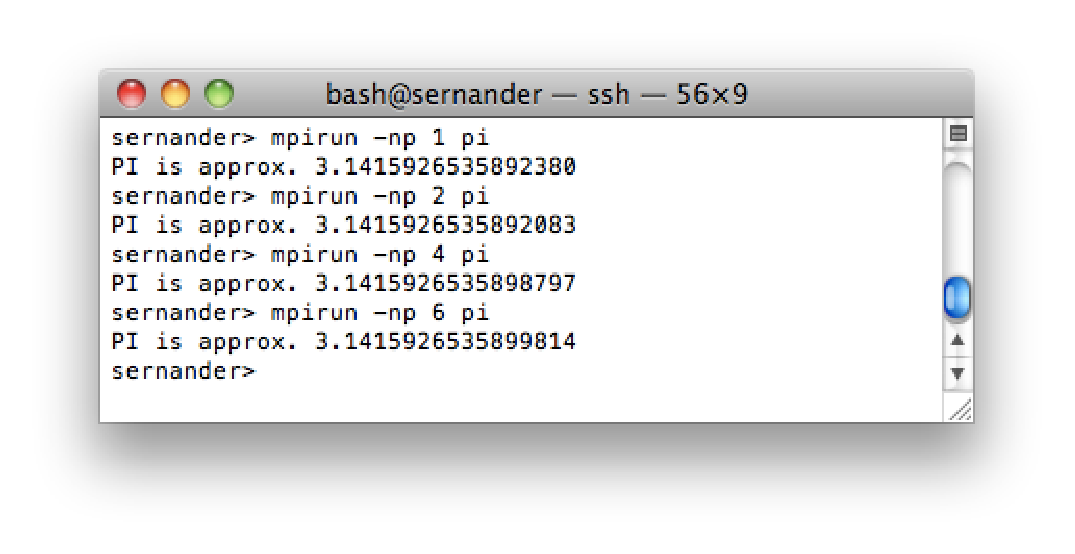
\includegraphics[width=\textwidth]{pic/pi.eps}
	\caption{Value of $\pi$ on a different number of processors}
\end{center}
\end{figure}

The results are a correct approximation of $\pi$, proof that the program does what it is designed for.


\clearpage
\chapter{Derived datatypes}

The function \textit{MPI\_Type\_vector} allows the user to create a derived datatype. In our case, we want to create a datatype representing the quater of a matrix having \textit{nx} lines and \textit{ny} columns.

The main parameters are defined as follows (given a type for the elements in the array, like \textit{MPI\_Double} in our case):
\begin{description}
	\item[count:] indicates the number of blocks in our datatype
	\item[blocklength:] indicates the length of a block
	\item[stride:] indicates the number of elements between the beginning of each block
\end{description}
So, when we will ask the system to transer such a datatype, it will transfer \textit{count} blocks of \textit{blocklength} elements, the first element of each block being separated from the next one by \textit{stride} elements. Thus, using the values \textit{count} = \textit{nx}/2, \textit{blocklength} = \textit{ny}/2 and \textit{stride} = \textit{ny}, we get a derived datatype representing a quater of our matrix.

The result of the program being huge, it has not been included here.


\clearpage
\input{q6}

%\newpage
%\setcounter{page}{1}
%\pagenumbering{Roman}
%\appendix
%\chapter{Point-to-point}

\section{Exchange.c}
\lstinputlisting{../code/exchange.c}

\section{Ping pong}
\lstinputlisting{../code/pingpong.c}

\chapter{Collective communication}

\section{pass-on}
\lstinputlisting{../code/onetoall.c}

\section{fan-out}
\lstinputlisting{../code/fanout.c}

\section{onetoall\_glob}
\lstinputlisting{../code/onetoall_glob.c}

\chapter{Reduction}

\lstinputlisting{../code/pi.c}

\chapter{Derived datatype}

\lstinputlisting{../code/datatypes.c}

\chapter{Communicators}

\lstinputlisting{../code/communicators.c}


\end{document}
